\documentclass[12pt]{article}

\usepackage{amsmath}
\usepackage{amssymb}
\usepackage{cmbright}
\usepackage{sfmath}
\usepackage{graphicx}
\usepackage[T1]{fontenc}
\usepackage{float}
\usepackage{hyperref}

\usepackage[backend=biber,style=authoryear,
	maxcitenames=1,uniquelist=false,uniquename=false]{biblatex}
\addbibresource{references.bib}

\begin{document}

\title{Summary of the last week}
\author{Kamal Ahmadov}
\date{\today}
\maketitle

\section{Analytical and semi-analytical solution of diffusion equation with ramp injection rate
  $q(t)=m_{\mathsf{q}}t$}

The governing aperture equation is the following PDE
\begin{equation}\label{pde}
	a \frac{ \partial }{ \partial x } \left(w^{n} \frac{ \partial w }{ \partial
		x }  \right)  = \frac{ \partial w }{ \partial t }.
\end{equation}
I consider a linearly increasing injection rate
\begin{equation}
	- a w^n \frac{ \partial w }{ \partial x }  = m_{\mathsf{q}} t
\end{equation}
\subsection{Closed-form solution for $n=0$}
Considering $n=0$, the dimensionless self-similar variables can be found to be
\begin{equation}\label{sim-variables}
	\theta(\zeta) = \frac{w(x,t) - w_{\mathsf{i}}}{m_{\mathsf{q}} \sqrt{ t / D }},
	\quad \zeta = \frac{x}{\sqrt{ D t }}
\end{equation}
where $\theta$ is dimensionless aperture, $\zeta$ is dimensionless
distance, and $D$ is the hydraulic diffusivity.

Replacing the variables in Eq. \ref{pde} with self-similar variables
(\ref{sim-variables}), I obtain the ODE
\begin{equation}\label{ode}
	\theta'' + \frac{\zeta}{2} \theta' - \frac{3}{2} \theta = 0
\end{equation}
with the injection condition
$$
	\theta'(0) = -1
$$
This equation is a special case of the family $L_{n}[f] := f'' + \frac{x}{2} f'
	- \frac{n}{2} f = 0$ where $n=3$. Differentiating this equation drops $n$ by 1
each time. So, differentiating Eq. \ref{ode} three times and replacing $\theta''' =
	g$ gives
$$
	g'' + \frac{\zeta}{2}g' = 0.
$$
It is now easy to find that the general solution for $g$ is
$$
	g(\zeta) = A \operatorname{erfc} (\zeta/2) + B.
$$
We can now integrate $g$ three times and apply the boundary conditions to obtain
the specific solution for $\theta$
\begin{equation}\label{ode-sol}
	\theta(\zeta) = \frac{\zeta^{2} + 4}{3 \sqrt{ \pi }} e^{ - \zeta^{2} / 4 } -
	\frac{\zeta^{3} + 6 \zeta}{6} \operatorname{erfc} (\zeta / 2)
\end{equation}

\subsection{Semi-analytical solution $n=3$}

Similar exercise can be done $n=3$, but the obtained ODE is a nonlinear ODE
whose closed-form solution does not exist. I instead solve it numerically using
\verb|scipy.integrate.solve_ivp| together with \verb|scipy.optimize.newton| to
find the second initial condition.

\subsection{Comparison between $n=0$ and $n=3$}

Figure \ref{fig:similarity-profiles} clearly shows the distinction in the shape
of profiles between rigid and soft cases. As expected, soft case exhibits a sharp front.

\begin{figure}[H]
	\centering
	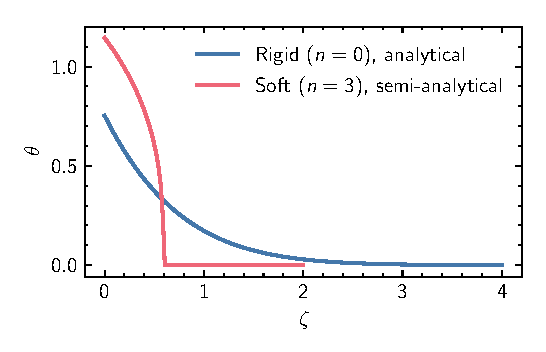
\includegraphics[width=0.95\textwidth]{figures/similarity-profiles.eps}
	\caption{Analytical and semi-analytical solutions of dimensionless aperture
		for $n=0$ and $n=3$, respectively.}
	\label{fig:similarity-profiles}
\end{figure}


\section{Aperture propagation along a long fracture with length $L=\mathsf{2\ km}$ shows the
  transition from rigid at small-times to soft behavior at large-times}

We already know that there exists a characteristic time $t_{\mathrm{c}}$ below
which the fracture behaves as rigid and above which the behavior is soft. We
have previously seen this transitional behavior across several simulation with
varying injection rates. The objective here is to achieve the transition between
the two regimes in a single simulation with a much longer fracture.

Figure \ref{fig:long-fracture-v1} shows this transition from rigid to soft
behavior along a 2 km fracture. At small times the aperture profiles are
smooth, similar to $n=0$ profile in Fig. \ref{fig:similarity-profiles}. And at
large times, there exists a sharp front ($n=3$ profile in Fig.
\ref{fig:similarity-profiles}). The comparison of the first few aperture profiles
with the exact solution for $n=0$ (Eq. \ref{ode-sol}) confirms the rigid
behavior of the fracture at small times.

\begin{figure}[H]
	\centering
	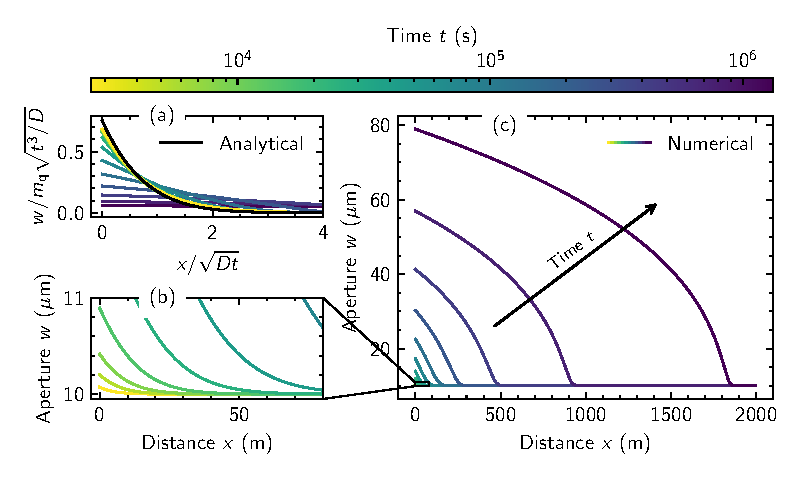
\includegraphics[width=0.95\linewidth]{figures/ramp-profiles-similarity-v2.eps}
	\caption{Aperture propagation along a long fracture shows the transition
		from smooth profiles at small times to the development of a sharp front at
		large times. (c) Aperture profiles along the fracture at different time steps.
		(b) Zoom into small times. (c) Comparison with the closed-form solution for
		dimensionless aperture with $n=0$ (Eq. \ref{ode-sol})}
	\label{fig:long-fracture-v1}
\end{figure}

Figure \ref{fig:long-fracture-v2} is a variant of Figure \ref{fig:long-fracture-v1}
that additionally compares the numerical profiles with the $n=3$ profile from
Figure \ref{fig:similarity-profiles}. Although the large-time dimensionless
aperture profiles do not fully collapse onto the $n=3$ profile, they clearly
approach it. A closer match requires a larger aperture at the injection
point.

\begin{figure}[H]
	\centering
	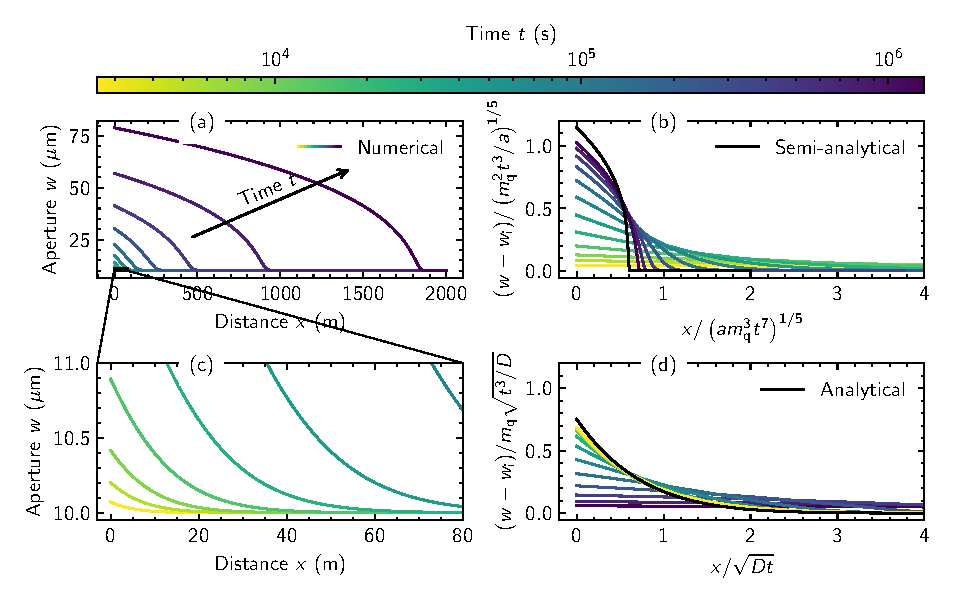
\includegraphics[width=0.95\linewidth]{figures/ramp-profiles-similarity-v3.eps}
	\caption{Similar to Figure \ref{fig:long-fracture-v1} but with an additional
		pane showing the (b)
		comparison to $n=3$ dimensionless aperture profile from Figure
		\ref{fig:similarity-profiles}.}
	\label{fig:long-fracture-v2}
\end{figure}


\section{Field hydraulic data}

\subsection{Soultz 1993 hydraulic stimulation}
Below is the figure \ref{fig:soultz-hydraulic} of wellhead pressure and flow rate evolution during Soultz
1993 hydraulic stimulation. Visual comparison with reference values from
\textcite{CornetEtAl2007} supports the validity of the data used here.

\begin{figure}[H]
	\centering
	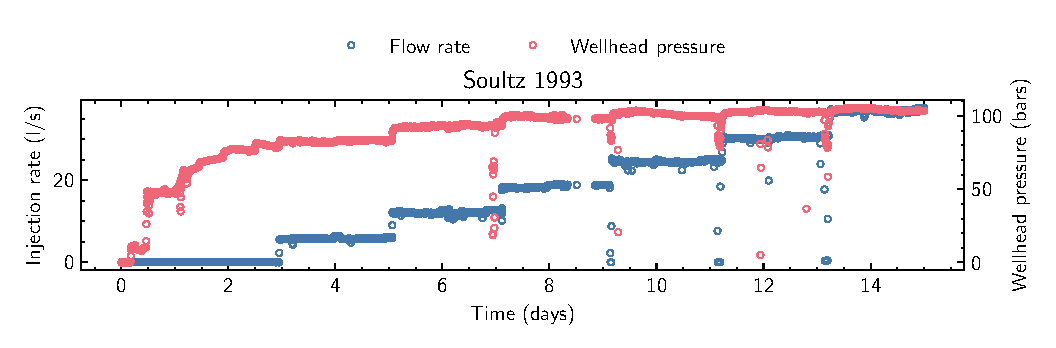
\includegraphics[width=0.95\linewidth]{figures/soultz-hydraulic.eps}
	\caption{Injection flow rate and wellhead pressure evolution with time
		during Soultz 1993 hydraulic stimulation}
	\label{fig:soultz-hydraulic}
\end{figure}

We have previously seen that our model also predicts a transitional behavior for
the evolution of pressure at the injector. It is therefore interesting to see if
a similar behavior is observed in the field. Figure \ref{fig:soultz-pressure}
shows the evolution of wellhead pressure in log scale at Soultz 1993. The
log-scale plot shows that the power-law behavior changes sharply several times
during the stimulation, but the dominant power-law behavior is probably $p \sim
	t^{0.2}$. Our model predicts $p \sim t^{3/2}$ at small times and $p \sim
	t^{3/5}$ at large times.

\begin{figure}[H]
	\centering
	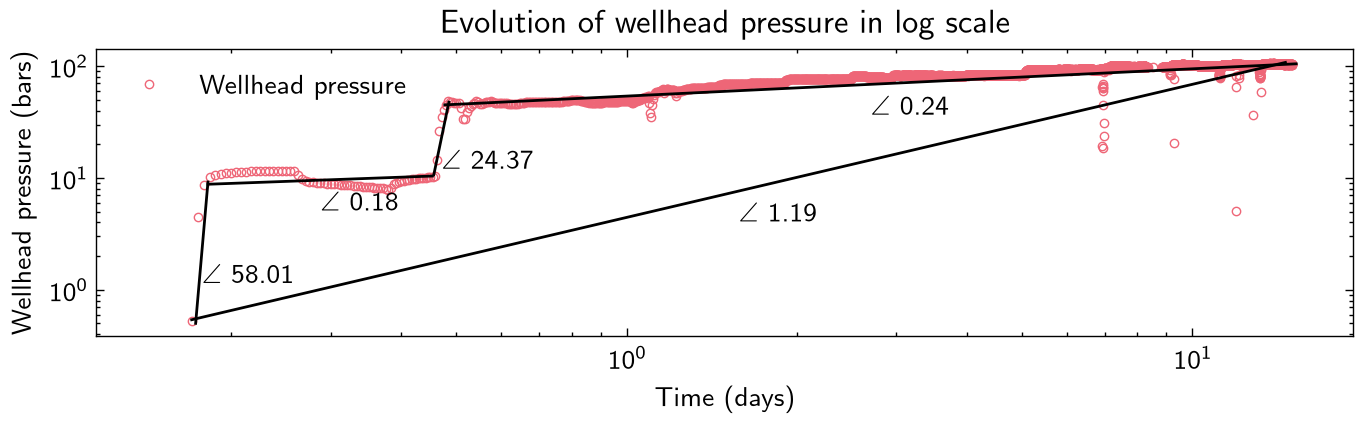
\includegraphics[width=0.95\linewidth]{figures/soultz-pressure.png}
	\caption{Wellhead pressure evolution in log scale together with slopes
		showing the power-law exponents at different time intervals}
	\label{fig:soultz-pressure}
\end{figure}

Figure \ref{fig:soultz-rate} shows that a linearly increasing injection rate
condition is a good approximation of the flow rate history of Soultz 1993
hydraulic stimulation. The slope is $m_{\mathsf{Q}}=\mathsf{3.2 \times 10^{-5}\
l/s^{2}}$.

\begin{figure}[H]
	\centering
	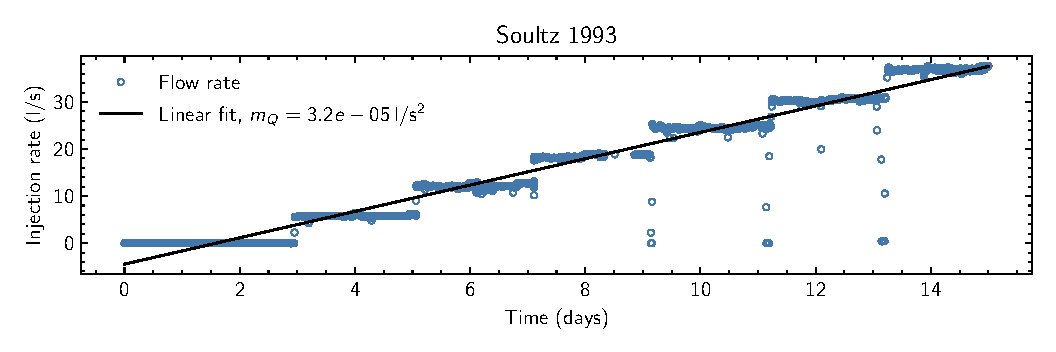
\includegraphics[width=0.95\linewidth]{figures/soultz-rate.eps}
	\caption{Linearly increasing injection rate with $m_{\mathsf{Q}}=\mathsf{3.2
				\times 10^{-5}\ l/s^{2}}$ fits well the injection flow rate history of
		Soultz 1993 hydraulic stimulation}
	\label{fig:soultz-rate}
\end{figure}

\subsection{Basel 2006 hydraulic stimulation}

I could not find the hydraulic data of Basel 2006 hydraulic stimulation. But
a fast skim of the literature \parencite{HaringEtAl2008,OrtizREtAl2011} suggests
that $p \sim t^{1/4}$. This power-law relationship is interpreted as being the
result of ``bilinear-flow''.

\printbibliography

\end{document}
